\documentclass[a4paper]{article}
\usepackage{tikz} 
\usepackage{array}
\usepackage{standalone}


\title{}
\author{}
\date{}


\begin{document}

\section{Introduction}
Cultural evolution theories provide a set of methods that can be used to account these dynamic of changes, focused on the production of olive oil amphorae during the Roman Empire. 
To achieve this goal, multivariate methods were used to evaluate the differences on the pattern production among pottery workshops. \\
Specifically we want to identify the origin of these changes and if these changes were produced by cultural reasons depending on the spatial distance and other cultural constraints. As hypothesis, we propose that spatial distribution of pottery workshops is the main influence of the making techniques processes \cite{schillinger}. Four pottery workshops, showed in the map \textbf{(fig.1)} were studied from different spaces in \emph{Baetica}. 
\begin{figure}[h!]
    \centering
    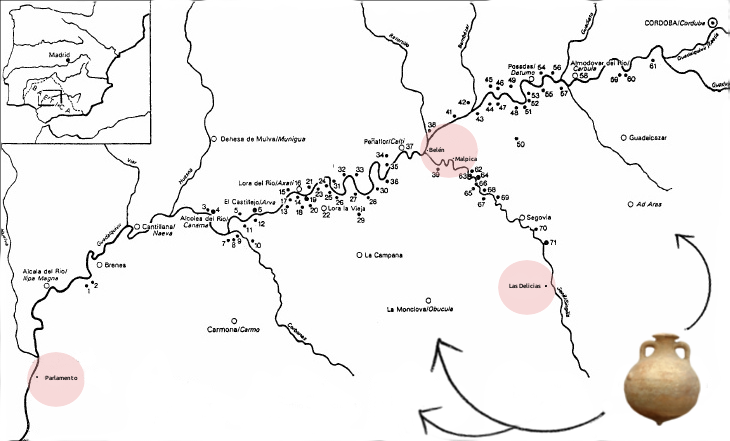
\includegraphics[width=0.6\linewidth]{images/fig1.png}
    \caption{Distribution map of the four amphorae workshops. The names are Las Delicias (\'Ecija, Seville), Bel\'en and Malpica (Palma del R\'io, C\'ordoba) and Parlamento (Seville)}

\end{figure}

\section{Empirical Studies}
\subsection{Methods}

{\textbf{Measurements}} \\

To explore the dynamic of changes we analysed a set of measures among different kinds of amphorae shapes from different workshops. We analysed 413 samples of amphorae from 4 different workshops. These workshops were selected from different spaces of \emph{Baetica} area in order to know if there were differences depending on the space. A database was created using a selection of 80 to 90 samples from each pottery workshops. In each sample of amphora we measured eight measurements among different part of the rim being focused on the rim of the amphora. 


In each sample of amphora we measured eight measurements among different part of the rim being focused on the rim of the amphora.

{\textbf{Multivariate method}} \\

Multivariable methods were used to explore these metrical observations \cite{li}

with the eight measurements as variables.\\ 
Principal Component Analysis allowed us to simplify the dataset to see which variable were more relevant. 
Our results suggested that first and second principal component were more relevant than the rest. 
\subsection{Results}

Several multivariate methods were used such as Principal Component Analysis and Discriminant Analysis to classify. These methods allowed us to know the differences on the pattern production among workshops.In our case, the first two principal components were taken to see the significal differences among workshops depending on the space. The \textbf{figure 2} shows the workshops with a minor space such Bel\'en and Malpica share more pottery traits than the rest: Parlamento and Las Delicias.

\begin{figure}
    \centering
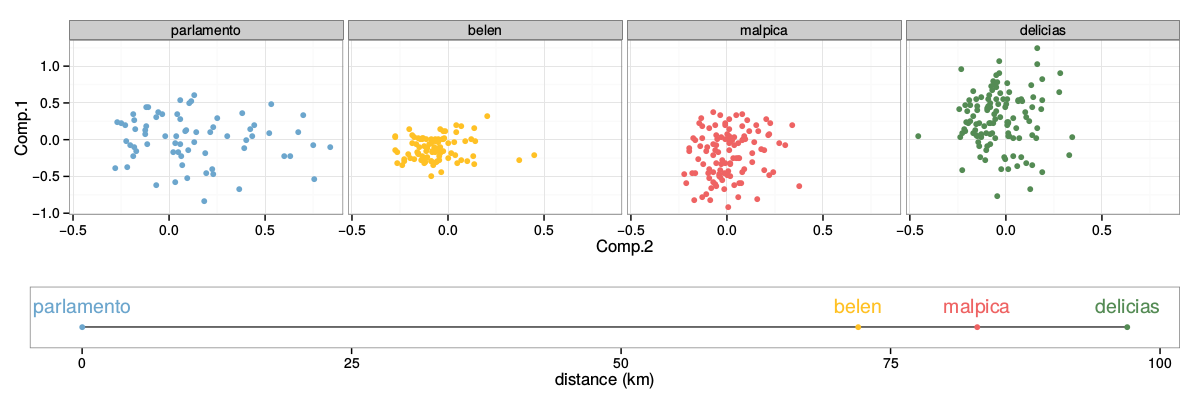
\includegraphics[width=0.7\linewidth]{images/fig2.png}
\caption{Plot with the results of the first two principal components given by the PCA}
\end{figure}

Once defined the components, we used Discriminant Analysis to find a combination among them to define the groups as well as possible. These results were translated to a confusion matrix which basically means what results were predicted as true or false on the discriminant analysis. 

 Thus the system had troubles to distinguishing between Bel\'en and Malpica which had a higher number of confusion or number instead of Parlamento with a minor confusion than the rest. 

 
\begin{figure}
    \centering
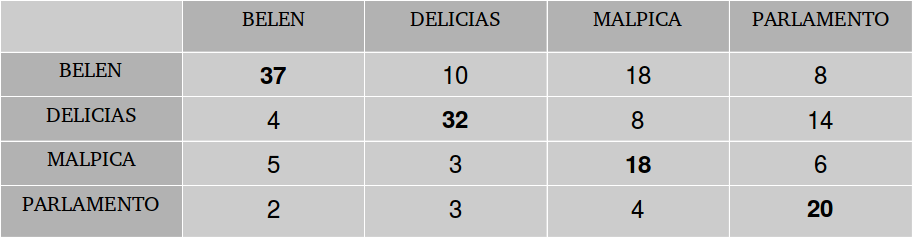
\includegraphics[width=0.6\linewidth]{images/fig3.png}
\caption{Matrix of confusion. Accuracy: 0.5573. P-Value: 0.0006991.}
\end{figure}

As shown in the \textbf{figure 3} of confusion, all correct guesses were located in the diagonal of the table.\\
A peer to peer comparison was developed among different workshops. We calculated the geographical distance between each site and the distance among pottery measures, calculated using the previous results. The \textbf{figure 4}  shows that the pottery distance is correlated with the spatial distance of workshops.  

\begin{figure}
    \centering
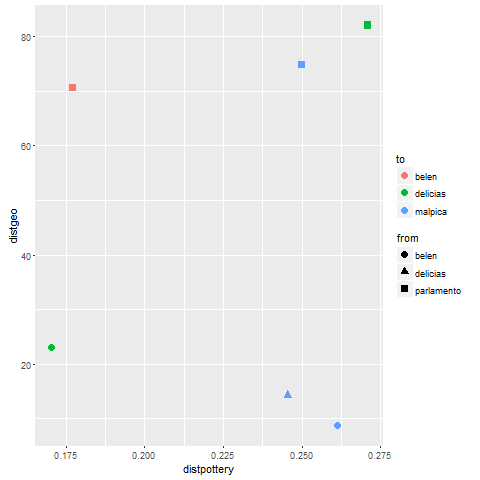
\includegraphics[width=0.7\linewidth]{images/fig4.png}
\caption{Distance metrics calculated among different workshops.}
\end{figure}

This suggest some cultural transimission with isolation by distance 



\section{Theoretical Exploration}
\subsection{Model}
We propose a simple model where a fixed number of workshop are producing a fixed amount of amphora during a certain time. 

To simplify the problem the amphora production is describe by only one mesure amoung the mesure previoulsy observerd (external diamater) and each workshop produce amphora where this measure follow a normal distribution. The paramater of this noraml distribution (the mean value and the standard deviation) are the cultural knowledge that workshop can or cannot exchange given the different setup. Every 100 timestep each workshop have a certain probability to modify those parameter and/or to copy the one used by another workshop. 



\subsection{Experimental Setup}
We create 4 different experimental setup that help us to test the impact of the horizontal transmission on the evolution of the variation in production of amphora given different penalities between each workshop. In two case the vertical transmission (\emph{ie} the copy of the paramater of the normal distribution) (left column of the Figure~\ref{fig:setmodel} are impossible; in the two other case (right column) yes. In two case the distance between two adjacent workshops is the same (top row of Fig~\ref{fig:setmodel}), in two other case (bottom row) no.
\begin{figure}[h!]
    \centering
    \begin{tabular}{m{4cm}m{4cm}}
	{\tiny No Horizontal Transmission} & {\centering\tiny Horizontal Transmission }\\
	\resizebox{4cm}{!}{
	    \documentclass{standalone}

\begin{document}
	    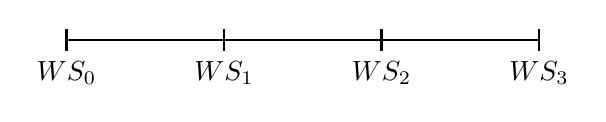
\begin{tikzpicture}[thick,scale=2]
		\coordinate (WS0) at (0,0);
		\coordinate (WS1) at (1,0);
		\coordinate (WS2) at (2,0);
		\coordinate (WS3) at (3,0);
		\draw[thick,-] (0,0) -- (3,0) node[anchor=north west] {};   
		\foreach \x in {0,1,2,3}
		\draw (\x cm,2pt) -- (\x cm,-2pt) node[anchor=north] {$WS_\x$};

	    \end{tikzpicture}
\end{document}



	}
	&
	\resizebox{4cm}{!}{
	    \documentclass{standalone}

\begin{document}
    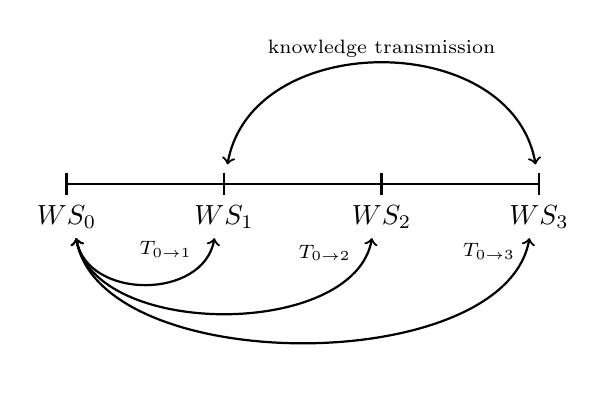
\begin{tikzpicture}[thick,scale=2]
		\coordinate (WS0) at (0,0);
		\coordinate (WS1) at (1,0);
		\coordinate (WS2) at (2,0);
		\coordinate (WS3) at (3,0);
		\draw[thick,-] (0,0) -- (3,0) node[anchor=north west] {};   
		\foreach \x in {0,1,2,3}
		\draw (\x cm,2pt) -- (\x cm,-2pt) node[anchor=north] {$WS_\x$};


		\draw [black,shorten <= 0.25cm, shorten >= 0.25cm, <->] (WS1) to[out=80,in=100,distance=1cm] node[above,font=\scriptsize]{knowledge transmission} (WS3); 


	\draw [black,shorten <= 0.7cm, shorten >= 0.7cm, <->] (WS0) to[out=-80,in=-100,distance=.75cm	]  node[font=\scriptsize,pos=.60	,above]{$T_{0 \rightarrow 1}$} (WS1);
	\draw [black,shorten <= 0.7cm, shorten >= 0.7cm, <->] (WS0) to[out=-80,in=-100,distance=1cm	]  node[font=\scriptsize,pos=.75	,above]{$T_{0 \rightarrow 2}$}(WS2);
	\draw [black,shorten <= 0.7cm, shorten >= 0.7cm, <->] (WS0) to[out=-80,in=-100,distance=1.25cm	]  node[font=\scriptsize,pos=.82		,above]{$T_{0 \rightarrow 3}$}(WS3);

    \end{tikzpicture}

\end{document}


	}\\
	\resizebox{4cm}{!}{
	    \documentclass{standalone}

\begin{document}
	    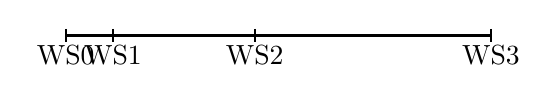
\begin{tikzpicture}[thick,scale=.6]
		\coordinate (WS0) at (0,0);
		\coordinate (WS1) at (1,0);
		\coordinate (WS2) at (4,0);
		\coordinate (WS3) at (9,0);
		\draw[thick,-] (0,0) -- (9,0) node[anchor=north west] {};   
		\foreach \x in {0,1,4,9}
		\draw (\x cm,4pt) -- (\x cm,-4pt) node[anchor=north] {};
		\draw (WS0) node[anchor=north]{WS0};
		\draw (WS1)node[anchor=north]{WS1};
		\draw (WS2)node[anchor=north]{WS2};
		\draw (WS3)node[anchor=north]{WS3};
	    \end{tikzpicture}
\end{document}


	}	&
	\resizebox{4cm}{!}{
	    
\documentclass{standalone}

\begin{document}
	    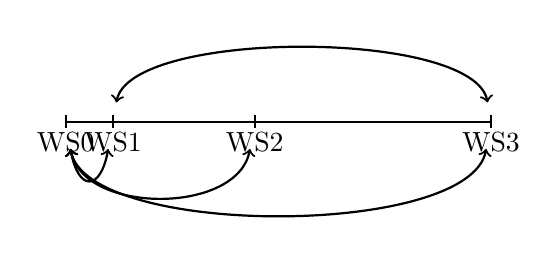
\begin{tikzpicture}[thick,scale=.6]
		\coordinate (WS0) at (0,0);
		\coordinate (WS1) at (1,0);
		\coordinate (WS2) at (4,0);
		\coordinate (WS3) at (9,0);
		\draw[thick,-] (0,0) -- (9,0) node[anchor=north west] {};   
		\foreach \x in {0,1,4,9}
		\draw (\x cm,4pt) -- (\x cm,-4pt) node[anchor=north] {};
		\draw (WS0) node[anchor=north]{WS0};
		\draw (WS1)node[anchor=north]{WS1};
		\draw (WS2)node[anchor=north]{WS2};
		\draw (WS3)node[anchor=north]{WS3};

		\draw [black,shorten <= 0.25cm, shorten >= 0.25cm, <->] (WS1) to[out=80,in=100,distance=2cm] (WS3); 
		\draw [black,shorten <= .35cm, shorten >= .35cm, <->] (WS0) to[out=-80,in=-100,distance=1.5cm	]  (WS1);
		\draw [black,shorten <= .35cm, shorten >= .35cm, <->] (WS0) to[out=-80,in=-100,distance=2cm	]  (WS2);
		\draw [black,shorten <= .35cm, shorten >= .35cm, <->] (WS0) to[out=-80,in=-100,distance=2.5cm	]  (WS3);
	    \end{tikzpicture}
\end{document}


	}	
    \end{tabular}
	\caption{Four different experimental Setup}
	\label{fig:setmodel}
\end{figure}


\subsection{Results}
We run 100 simulation for each setup during $10\,000$ steps. For each simulation and at every 1000 timestep we mesure the mean of the selected measure of the amphora for each workshop and we calculate the standard deviation of this mean \emph{between} all the workshop. The Figure~\ref{fig:resmod} show the evolution of  this standard deviation for all the simulation in each experimental setup.
    \begin{figure}[h!]
    \centering
	\begin{tabular}{m{4cm}m{4cm}}
	    {\tiny \hspace{.4cm}No Horizontal Transmission} & {\centering\tiny Horizontal Transmission }\\
	    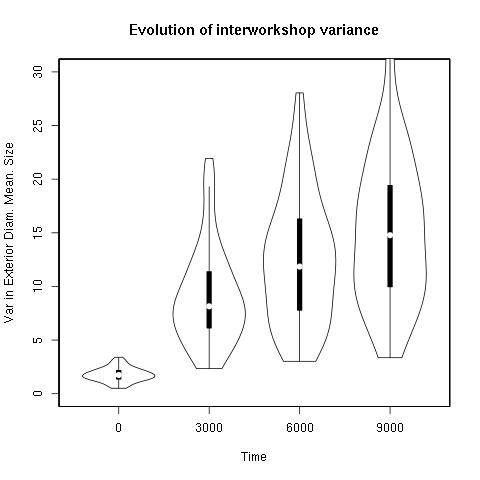
\includegraphics[height=4cm]{images/lineNC.png}
	    &
	    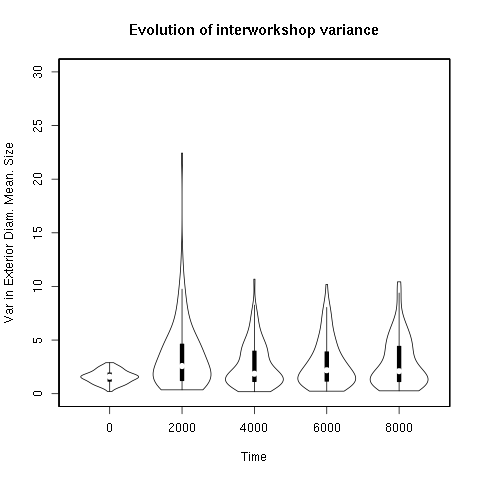
\includegraphics[height=4cm]{images/lineC.png}\\
	    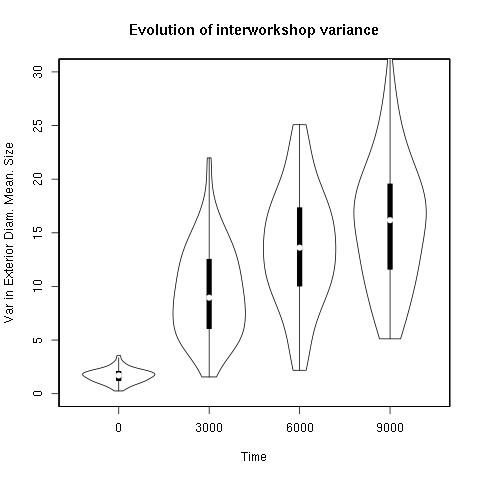
\includegraphics[height=4cm]{images/cubeNC.png}
	    &
	    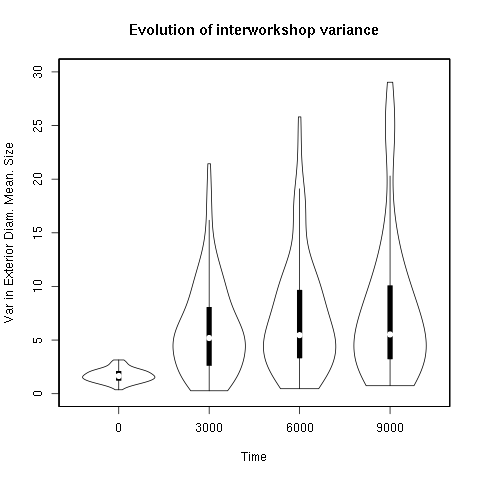
\includegraphics[height=4cm]{images/cubeC.png}\\
	\end{tabular}
	\caption{Evolution of the variation of the mean of the observed measure between the workshops}
	\label{fig:resmod}
    \end{figure}

    We observe that in the cases without vertical transimssion the variation between the mean of the mesure grows, as every workshop wil slowly change is way to produce amphora without interacting with the other. In the two other case, if all the workshops are close enough, the cultural transmission of knowledge will leave the variation between the worksop at a same level. In order to have an increase of the variation in production technics between the amphora, some strong obstacle in transmission such has a high cost of travel, has to be introduce.

    \section{Conclusion}
    
    This suggest that
 


\begin{thebibliography}{50}
	\bibitem[1]{mesoudi}\textsc{Mesoudi, A. (2015)}
	\textit{Cultural Evolution: A review of Theory, Finding and Controversies}, Evolutionary biology.

	\bibitem[2]{agui}\textsc{Aguilera, A. (1998)}
	\textit{An\'alisis multivariable: una nueva v\'ia para la caracterizaci\'on cer\'amica}, Pyranae, 29.

	\bibitem[3]{schillinger}\textsc{Schillinger, K. et al. (2006)}
	\textit{Differences in Manufacturing Traditions and Assemblage-Level Patterns: the Origins of Cultural Differences in Archaeological Data}, Journal of Archaeological Method Theory.

	\bibitem[4]{li}\textsc{Li, A. (2014)}
	\textit{Crossbows and imperial craft organisation: the bronze triggers of China's Terracotta Army}, Antiquity, 88.339.

\end{thebibliography}

\end{document}




